\chapter{Power System - Censnet} \label{cap:mpcc}

\section{Preliminaries}

\subsection{Graph definition}


A \textbf{graph} $G$ is a mathematical structure that represents a set of interconnected objects. These objects are known as \textbf{vertices} (or \textbf{nodes}), denoted by the set $V(G)$, and the connections between them are called \textbf{edges} (or \textbf{arcs}), denoted by the set $E(G)$. Formally, a graph is defined as an ordered pair $G = (V, E)$, where $V(G)$ is a non-empty set of vertices, and $E(G) \subseteq \{(u, v) \mid u, v \in V(G), u \neq v\}$ is a set of edges, where each edge connects two distinct vertices.

Graphs can be categorized based on the properties of their edges. An \textbf{undirected graph} has edges that do not have a direction, so the pair $(u, v) = (v, u)$ represents an edge that simply connects vertices $u$ and $v$. In contrast, in a \textbf{directed graph} (or \textbf{digraph}), each edge $(u, v) \in E(G)$ has a direction, meaning it goes from vertex $u$ to vertex $v$. This implies that $(u, v) \neq (v, u)$ unless $u = v$

 %
% \begin{figure}
%     \begin{center}
%         \setlength\figurewidth{.5\textwidth}        
%             \setlength\figureheight{0.4\textwidth}
%         \resizebox{\figurewidth}{\figureheight}{\input{figures/Chapter_LinealCensnet/graph_def}}
%         % \input{figures/Chapter_LinealCensnet/graph_def}
%         % \includegraphics[width=0.95\textwidth]{figures/}
%     \end{center}
%     \caption{Directed graph}\label{fig:graph_definition}
% \end{figure}
%
\begin{figure}
    \centering
        \setlength\figurewidth{.5\textwidth}        
        \setlength\figureheight{0.4\textwidth} 
        \subfloat [Undirected graph] {\label{fig:undirected_graph_def}\resizebox{\figurewidth}{\figureheight}{\begin{tikzpicture}[>=Stealth, node distance=5cm]
    
    % Define styles for the nodes and edges
    \tikzstyle{node_style}=[circle, draw, minimum size=.9cm, inner sep=0pt, font=\normalsize]
    \tikzstyle{edge_style}=[draw, -, thick]

    % Nodes
    \node[node_style] (n1) {1};
    \node[node_style] (n2) [right of=n1] {2};
    \node[node_style] (n3) [right of=n2] {3};
    \node[node_style] (n4) [below of=n2] {4};

    % Edges with labels
    \draw[edge_style] (n1) edge node[above] {A} (n2);
    \draw[edge_style] (n4) edge node[left] {B} (n1);
    \draw[edge_style] (n4) edge node[right] {C} (n2);
    \draw[edge_style] (n3) edge node[right] {D} (n4);
    \draw[edge_style] (n1) to[out=30, in=150] node[above] {E} (n3);
    \draw[edge_style] (n3) edge node[above] {F} (n2);

\end{tikzpicture}
}}
        \subfloat [Directed graph] {\label{fig:direc_graph_def}\resizebox{\figurewidth}{\figureheight}{\input{figures/Chapter_LinealCensnet/di_graph_def}}}
        % \includegraphics[width=0.45\textwidth]{figures/}
    \caption{Types of graphs}\label{fig:graph_definition}
\end{figure}

In \Cref{fig:graph_definition}, two graphs are represented, each composed of four nodes labeled $1$, $2$, $3$, and $4$,, and six edges labeled $A$, $B$, $C$, $D$, $E$, and $F$. The difference between them lies in the type of graph they represent. For example, in \Cref{fig:undirected_graph_def}, the edge c shows a connection between nodes 2 and 4. However, in \Cref{fig:direc_graph_def}, this connection provides additional information: a direction, which, in the context of this study, could represent the direction of a specific element, such as electric power or flow.


A graph can be represented in various ways using matrices, each capturing different aspects of the graph's structure. The two most common matrix representations are the \textbf{adjacency matrix} and the \textbf{incidence matrix}.

The \textbf{adjacency matrix} of a graph is a square matrix used to represent the connections between vertices. For a graph $G$ with $n$ vertices, the adjacency matrix $A$ is an $n \times n$ matrix where the entry $a_{ij}$ is defined as follows:

\[
a_{ij} =
\begin{cases}
1 & \text{if there is an edge from vertex } i \text{ to vertex } j, \\
0 & \text{otherwise}.
\end{cases}
\]

For a directed graph, the adjacency matrix captures the direction of the edges. Below is the adjacency matrix for the directed graph shown earlier:

\[
A = \begin{pmatrix}
0 & 1 & 0 & 1 \\
1 & 0 & 0 & 1 \\
0 & 1 & 0 & 1 \\
1 & 1 & 1 & 0
\end{pmatrix}
\]


The \textbf{incidence matrix} of a graph represents the relationship between vertices and edges. For a graph $G$ with $n$ vertices and $m$ edges, the incidence matrix $I$ is an $n \times m$ matrix where the entry $i_{ij}$ is defined as follows:

\[
i_{ij} =
\begin{cases}
1 & \text{if vertex } i \text{ is the starting point of edge } j \text{ in a directed graph}, \\
-1 & \text{if vertex } i \text{ is the endpoint of edge } j \text{ in a directed graph}, \\
0 & \text{if vertex } i \text{ is not connected to edge } j.
\end{cases}
\]

For the directed graph previously described, the incidence matrix is given by:

\[
I = \begin{pmatrix}
1 & -1 & 0 & 0 \\
-1 & 0 & -1 & 0 \\
0 & 0 & 0 & 1  \\
0 & 1 & 1 & -1 
\end{pmatrix}
\]

\subsection{Neural networks}

\subsubsection{Multi-Layered Perceptrons}


A Multilayer Perceptron (MLP) is a fundamental type of artificial neural network, often regarded as one of the building blocks of deep learning. At its core, an MLP consists of multiple layers of nodes, or neurons, where each layer is fully connected to the next one. The architecture typically includes an input layer, one or more hidden layers, and an output layer. The neurons in each layer are connected to the neurons in the subsequent layer through weighted connections, which are the key parameters learned during the training process. One of the most significant properties of an MLP is its ability to function as a universal approximator. This means that, given sufficient neurons in the hidden layers, an MLP can approximate any continuous function to an arbitrary degree of accuracy, provided the network is trained properly.

Mathematically, an MLP can be defined as follows. Let $\mathbf{x} \in \mathbb{R}^n$ represent the input vector, where $n$ is the number of features. The output of each neuron in the first hidden layer is calculated as:

\[
\mathbf{z}^{(1)} = \sigma\left(\mathbf{W}^{(1)}\mathbf{x} + \mathbf{b}^{(1)}\right)
\]

where $\mathbf{W}^{(1)} \in \mathbb{R}^{m_1 \times n}$ is the weight matrix for the first hidden layer, with $m_1$ being the number of neurons in this layer, $\mathbf{b}^{(1)} \in \mathbb{R}^{m_1}$ is the bias vector, and $\sigma(\cdot)$ is the activation function, typically a non-linear function such as the ReLU (Rectified Linear Unit) or sigmoid function.

This process is repeated for each subsequent hidden layer $k$, where the output of the $k$-th layer is given by:

\[
\mathbf{z}^{(k)} = \sigma\left(\mathbf{W}^{(k)}\mathbf{z}^{(k-1)} + \mathbf{b}^{(k)}\right)
\]

Here, $\mathbf{W}^{(k)} \in \mathbb{R}^{m_k \times m_{k-1}}$ represents the weight matrix connecting layer $k-1$ to layer $k$, $\mathbf{b}^{(k)} \in \mathbb{R}^{m_k}$ is the bias vector for layer $k$, and $\mathbf{z}^{(k-1)}$ is the output of the previous layer.

Finally, the output layer produces the final prediction $\mathbf{\hat{y}}$:

\[
\mathbf{\hat{y}} = \sigma\left(\mathbf{W}^{(L)}\mathbf{z}^{(L-1)} + \mathbf{b}^{(L)}\right)
\]

where $L$ denotes the number of layers in the network, including the input and output layers. Depending on the nature of the problem (e.g., classification or regression), the activation function $\sigma(\cdot)$ used in the output layer can vary, with softmax being common in multi-class classification problems, and a linear activation for regression tasks.

The entire MLP is trained using a process called backpropagation, combined with an optimization algorithm like gradient descent, to minimize a loss function $J(\mathbf{y}, \mathbf{\hat{y}})$, which measures the difference between the true outputs $\mathbf{y}$ and the predicted outputs $\mathbf{\hat{y}}$.


\begin{figure}
    \centering
    \setlength\figurewidth{1\textwidth}        
    \setlength\figureheight{0.5\textwidth}
    \resizebox{\figurewidth}{\figureheight}{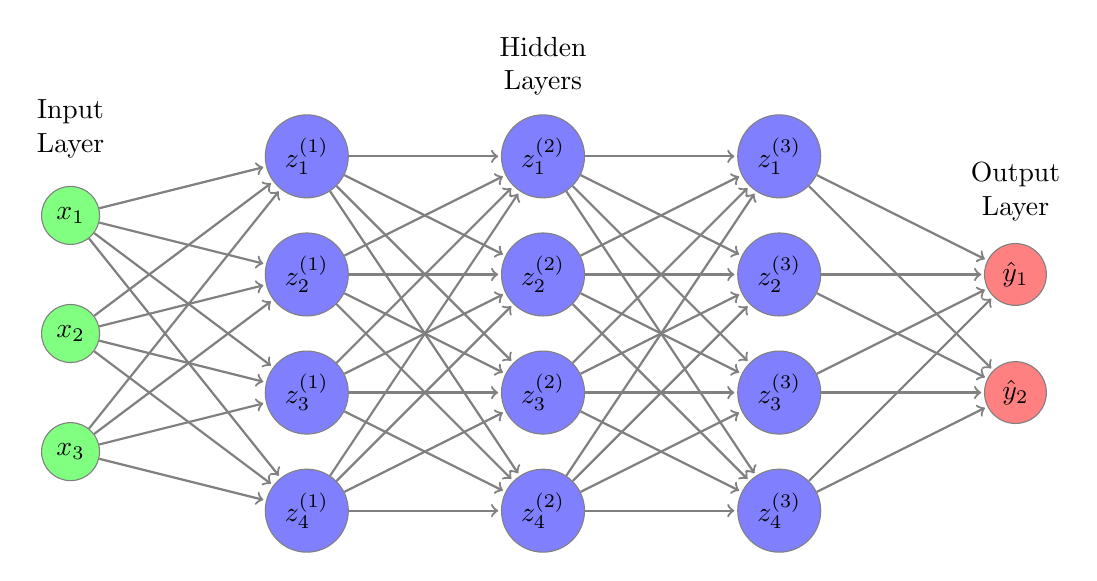
\begin{tikzpicture}[shorten >=1pt, ->, draw=black!50, node distance=1.5cm and 3.5cm, align=center]

    % Styles
    \tikzstyle{input} = [circle, draw, fill=green!50, minimum size=2em]
    \tikzstyle{hidden} = [circle, draw, fill=blue!50, minimum size=2em]
    \tikzstyle{output} = [circle, draw, fill=red!50, minimum size=2em]
    \tikzstyle{connection} = [->, thick]

    % Network Stage Labels
    \node[align=center] at (0,-0.4) {Input \\ Layer};
    \node[align=center] at (6,0.4) {Hidden \\ Layers};
    \node[align=center] at (12,-1.2) {Output \\ Layer};

    % Input Layer
    \foreach \i in {1,2,3}
        \node[input] (I\i) at (0,-\i*1.5) {$x_\i$};

    % Hidden Layer 1
    \foreach \i in {1,2,3,4}
        \node[hidden] (H1\i) at (3,-\i*1.5+0.75) {$z^{(1)}_\i$};

    % Hidden Layer 2
    \foreach \i in {1,2,3,4}
        \node[hidden] (H2\i) at (6,-\i*1.5+0.75) {$z^{(2)}_\i$};

    % Hidden Layer 3
    \foreach \i in {1,2,3,4}
        \node[hidden] (H3\i) at (9,-\i*1.5+0.75) {$z^{(3)}_\i$};

    % Output Layer
    \foreach \i in {1,2}
        \node[output] (O\i) at (12,-\i*1.5-0.75) {$\hat{y}_\i$};

    % Connections from Input to Hidden Layer 1
    \foreach \i in {1,2,3}
        \foreach \j in {1,2,3,4}
            \draw[connection] (I\i) -- (H1\j);

    % Connections from Hidden Layer 1 to Hidden Layer 2
    \foreach \i in {1,2,3,4}
        \foreach \j in {1,2,3,4}
            \draw[connection] (H1\i) -- (H2\j);

    % Connections from Hidden Layer 2 to Hidden Layer 3
    \foreach \i in {1,2,3,4}
        \foreach \j in {1,2,3,4}
            \draw[connection] (H2\i) -- (H3\j);

    % Connections from Hidden Layer 3 to Output Layer
    \foreach \i in {1,2,3,4}
        \foreach \j in {1,2}
            \draw[connection] (H3\i) -- (O\j);

\end{tikzpicture}
}
    % 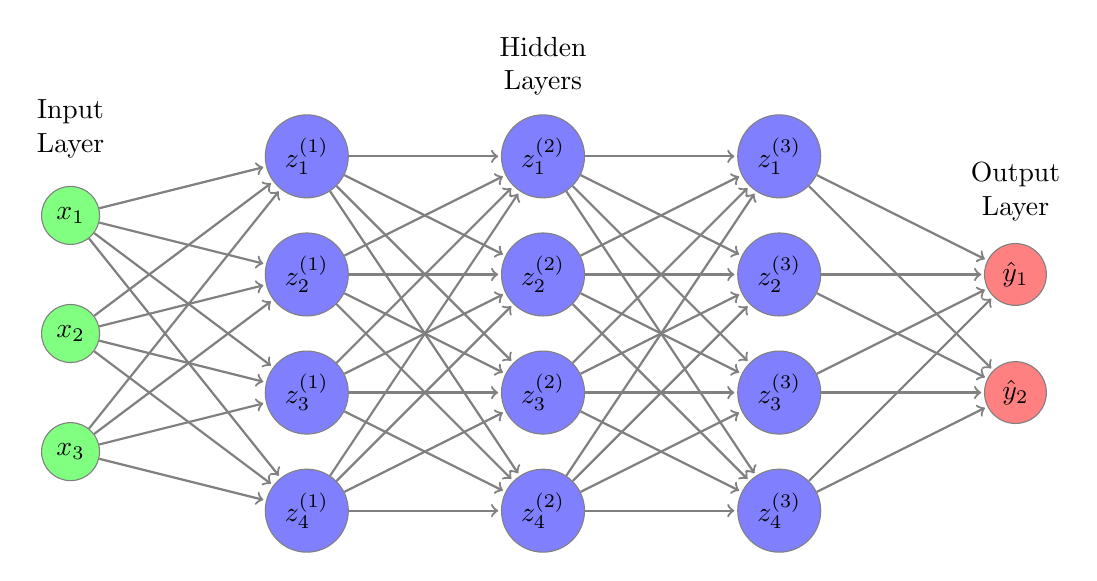
\begin{tikzpicture}[shorten >=1pt, ->, draw=black!50, node distance=1.5cm and 3.5cm, align=center]

    % Styles
    \tikzstyle{input} = [circle, draw, fill=green!50, minimum size=2em]
    \tikzstyle{hidden} = [circle, draw, fill=blue!50, minimum size=2em]
    \tikzstyle{output} = [circle, draw, fill=red!50, minimum size=2em]
    \tikzstyle{connection} = [->, thick]

    % Network Stage Labels
    \node[align=center] at (0,-0.4) {Input \\ Layer};
    \node[align=center] at (6,0.4) {Hidden \\ Layers};
    \node[align=center] at (12,-1.2) {Output \\ Layer};

    % Input Layer
    \foreach \i in {1,2,3}
        \node[input] (I\i) at (0,-\i*1.5) {$x_\i$};

    % Hidden Layer 1
    \foreach \i in {1,2,3,4}
        \node[hidden] (H1\i) at (3,-\i*1.5+0.75) {$z^{(1)}_\i$};

    % Hidden Layer 2
    \foreach \i in {1,2,3,4}
        \node[hidden] (H2\i) at (6,-\i*1.5+0.75) {$z^{(2)}_\i$};

    % Hidden Layer 3
    \foreach \i in {1,2,3,4}
        \node[hidden] (H3\i) at (9,-\i*1.5+0.75) {$z^{(3)}_\i$};

    % Output Layer
    \foreach \i in {1,2}
        \node[output] (O\i) at (12,-\i*1.5-0.75) {$\hat{y}_\i$};

    % Connections from Input to Hidden Layer 1
    \foreach \i in {1,2,3}
        \foreach \j in {1,2,3,4}
            \draw[connection] (I\i) -- (H1\j);

    % Connections from Hidden Layer 1 to Hidden Layer 2
    \foreach \i in {1,2,3,4}
        \foreach \j in {1,2,3,4}
            \draw[connection] (H1\i) -- (H2\j);

    % Connections from Hidden Layer 2 to Hidden Layer 3
    \foreach \i in {1,2,3,4}
        \foreach \j in {1,2,3,4}
            \draw[connection] (H2\i) -- (H3\j);

    % Connections from Hidden Layer 3 to Output Layer
    \foreach \i in {1,2,3,4}
        \foreach \j in {1,2}
            \draw[connection] (H3\i) -- (O\j);

\end{tikzpicture}

    \caption{}\label{fig:}
\end{figure}













\section{Linear formulation of the natural gas system} \label{sec:LinealCensnet_formulation}


Natural gas is a widely used energy resource, particularly for electricity generation. The natural gas system consists of a network of production centers, pipelines, compressor stations, storage facilities, and distribution points that ensure reliable gas delivery from producers to consumers. Mathematically, this system can be represented as a directed graph defined as $\mathcal{G}_f = \left\{\mathcal{N}_f, \mathcal{E}_f\right\}$ where $\mathcal{N}_f$ is the set of units within the gas system, and $ \mathcal{E}_f$ is the set of different elements linking them. This set of units includes gas supply nodes or wells $\mathcal{W} \subset \mathcal{N}_{f}$, gas demand nodes or users $\mathcal{U} \subset \mathcal{N}_{f}$, and gas storage facilities $\mathcal{S} \subset \mathcal{N}_{f}$. Similarly, the set of directed gas adjacency edges $\mathcal{A} = \left\{(n,m) \mid n,m\in\mathcal{N}_f \right\} \subset \mathcal{E}$ delineates the network structure through two kinds of transmission elements: transport pipelines $\mathcal{P} = \left\{p=(n,m) \mid n,m\in\mathcal{N}_f \right\}$ and compressing stations $\mathcal{C} = \left\{c=(n,m) \mid n,m\in\mathcal{N}_f \right\}$, so that $\mathcal{P}\cup\mathcal{C}=\mathcal{A}$ and $\mathcal{P}\cap\mathcal{C}=\emptyset$.


Natural gas transportation requires coordination to manage the flow through the different elements to maintain safe operating ranges. In optimizing this network, mathematical models minimize overall operating costs associated with the various stages of natural gas transportation, compression, storage, and handling unsupplied demand, ensuring compliance with technical and physical constraints. The function is expressed as:

\begin{equation} \label{eq:obj_func_integrated}
\begin{split}
\min_{\mathcal{P}, \mathcal{F}} \quad  \sum_{w \in \mathcal{W}} C_{w}^t {f_{w}^t} + \sum_{p \in \mathcal{P}} C_{p}^t {f_{p}^t} + \sum_{c \in \mathcal{C}} C_{c}^t {f_{c}^t} + \\ \sum_{u \in \mathcal{U}} C_{u}^{t} {f_{u}^{t}} + \quad \sum_{s \in \mathcal{S}} C_{s+}^{t} {f_{s+}^{t}}  + \sum_{s \in \mathcal{S}} C_{s-}^{t} {f_{s-}^{t}} + \sum_{s \in \mathcal{S}} C_{s}^{t} {V_{s}^{t}}
\end{split}
\end{equation}

The term $\sum_{w \in \mathcal{W}} C_{w}^t {f_{w}^t}$ represents the total cost of gas production at the wells, where $C_{w}^t$ denotes the cost per unit flow of gas at a specific well $w$ during time period $t$, and $f_{w}^t$ corresponds to the flow of gas from well $w$. Similarly, the transportation of gas through pipelines is captured by the term $\sum_{p \in \mathcal{P}} C_{p}^t {f_{p}^t}$, where $C_{p}^t$ is the cost per unit flow through pipeline $p$ during time period $t$, and $f_{p}^t$ represents the flow of gas through pipeline $p$. In addition, the total cost associated with gas compression at compressor stations is accounted for by $\sum_{c \in \mathcal{C}} C_{c}^t {f_{c}^t}$, where $C_{c}^t$ is the cost per unit flow at compressor station $c$ during time period $t$, and $f_{c}^t$ is the flow of gas through compressor station $c$.

Beyond production, transportation, and compression, the model also considers the costs related to unmet gas demand. The term $\sum_{u \in \mathcal{U}} C_{u}^{t} {f_{u}^{t}}$ reflects the penalty cost associated with unsupplied gas demand, where $C_{u}^{t}$ is the penalty cost per unit of unsupplied gas at location $u$ during time period $t$, and $f_{u}^{t}$ represents the volume of unmet demand. Additionally, the model includes costs related to storage operations. The term $\sum_{s \in \mathcal{S}} C_{s+}^{t} {f_{s+}^{t}}$ represents the cost of injecting gas into storage facilities, where $C_{s+}^{t}$ is the cost per unit flow into storage during time period $t$, and $f_{s+}^{t}$ denotes the flow into storage at facility $s$. Conversely, the cost of withdrawing gas from storage is captured by $\sum_{s \in \mathcal{S}} C_{s-}^{t} {f_{s-}^{t}}$, where $C_{s-}^{t}$ is the cost per unit flow out of storage during time period $t$, and $f_{s-}^{t}$ represents the flow out of storage at facility $s$. Finally, the model accounts for the storage cost itself through the term $\sum_{s \in \mathcal{S}} C_{s}^{t} {V_{s}^{t}}$, where $C_{s}^{t}$ is the cost per unit volume of gas stored at facility $s$ during time period $t$, and $V_{s}^{t}$ denotes the volume of gas stored. 


% Lastly, \Cref{eq:weymouth_cons}, known as the Weymouth equation, summarizes the physical behavior of gas flow through pipelines by relating the gas flow through the pipeline $f_{p}^t$ to the pressures at the ends of the pipeline $\pi_{n}^t, \pi_{m}^t \ \forall \ p = (n,m) \in\mathcal{P}$. The Weymouth equation defines a nonlinear, nonconvex, disjunctive flow-pressure relationship that hampers the optimization of the gas transport system.
% \begin{subequations}
\begin{alignat}{4}
    \underline{f_{w}^t} \leq f_{w}^t \leq \overline{f_{w}^t} &\quad \forall \ w \in \mathcal{W} \label{eq:well_limits} \\
    -\overline{f_{p}^t} \leq f_{p}^t \leq \overline{f_{p}^t} &\quad \forall \ p \in \mathcal{P} \label{eq:pipe_limits} \\
    % \underline{\pi_{n}^t} \leq \pi_{n}^t \leq \overline{\pi_{n}^t} &\quad \forall \ n \in \mathcal{N}_f \label{eq:press_limit} \\
    % \pi_{m}^t \leq \beta_{c}^t{\pi_{n}^t} &\quad \forall c=(n,m) \in \mathcal{C} \label{eq:comp_ratio} \\
    0 \leq f_{u}^{t} \leq \overline{f_{u}^{t}} &\quad \forall \ u \in \mathcal{U} \label{eq:dem_limit_gas} \\
    \sum_{m:(m,n)\in\mathcal{A}}{f_{m}^t} = \sum_{m':(n,m')\in\mathcal{A}}{f_{m'}^t} &\quad \forall \ n \in \mathcal{N}_f \label{eq:gas_balance} \\
    0 \leq f_{s+}^t \leq V_{0s} - \underline{V_s} &\quad \forall \ s \in \mathcal{S} \label{eq:sto_limit1} \\ 
    0 \leq f_{s-}^t \leq \overline{V_s} - V_{0s} &\quad \forall \ s \in \mathcal{S} \label{eq:sto_limit2} \\ 
    V_{s}^t = V_{s}^{t-1} + f_{s-}^{t-1} - f_{s+}^{t-1} &\quad \forall \ s \in \mathcal{S} \label{eq:sto_time}\\
    % sgn(f_{p}^t)(f_{p}^t)^2 = K_{nm}((\pi_{n}^t)^2-(\pi_{m}^t)^2) &\quad \forall \ p =(n,m) \in\mathcal{P} \label{eq:weymouth_cons}
\end{alignat}

The constraint set models the gas transportation system: \Cref{eq:well_limits} forces each production well to inject the flow $f_{w}^t$ over the technical minimum $\underline{f_{w}^t}$ and under the maximum capacity $\overline{f_{w}^t}$. \Cref{eq:pipe_limits} upper-bounds the gas flow through pipelines $f_{p}^t$ to the structural capacity $\overline{f_{p}^t}$. \Cref{eq:dem_limit_gas} ensures that the unsupplied demand $f_{u}^{t}$ is lower than the corresponding user demand $\overline{f_{u}^{t}}$. The nodal gas balance in \Cref{eq:gas_balance} guarantees that the gas entering the node $n$ equals the gas leaving it. \Cref{eq:sto_limit1,eq:sto_limit2} limit the gas injection $f_{s+}$  and extraction $f_{s-}$ rates at storage facilities according to the feasible operating range determined by the currently stored volume $V_{s}^t$, respectively. In turn, \Cref{eq:sto_time} balances the gas storage unit such that gas volume at operation period $t$ $V_{s}^t$ equals the volume from period $V_{s}^{t-1}$ plus the difference between injected $f_{s+}^{t-1}$ and extracted $f_{s+}^{t-1}$ gas flow, a fundamental constraint for modeling the dynamics of gas storage over time. 


